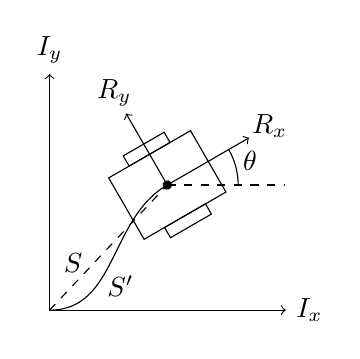
\begin{tikzpicture}[scale=3]
% axis labels
\node at (0,1.1) {$I_y$};
\node at (1.1,0) {$I_x$};

% inertial axis
\draw[<->] (0,1) -- (0,0) -- (1,0);

% robot reference frame
\begin{scope}[rotate around={30:(0.4,0.3)},shift={(0.4,0.3)}]
%wheels 
	\draw (.1,0) rectangle (.3,-0.05);
	\draw (.1,.3) rectangle (.3,.35);
	%robot body
	\draw (0,0) rectangle (0.4,0.3);
	% axis
	\coordinate (C) at (.2,0.15);
	\draw[fill=black] (C) circle [radius=0.05em];
	\draw[<->] (.2,.5) -- (.2,0.15) -- (0.6,0.15);
	% rotation angle
	\begin{scope}[rotate around={-30:(.2,0.15)},shift={(.2,0.15)},dashed]
		\draw[dashed] (0,0) -- (.5,0);
		\draw[solid] (0.3,0) arc [start angle=0,end angle=30, radius=.3];
		\node at (.35,0.1) {$\theta$};
	\end{scope}
	% axis labels
	\node at (.2,.6) {$R_y$};
	\node at (.7,.15) {$R_x$};
\end{scope}
% robot position line
\node at (.1,.2) {$S$};
\draw[-,dashed] (0,0) -- (C);
% robot curve line
\draw (0,0) to [out=0,in=210] (C);
\node at (.3,.1) {$S\mathrm{'}$};
\end{tikzpicture}
